%===================================== CHAP 5 =================================

\chapter{Sample Preparation and Polishing}
As the continued development of optical fibers, and fiber based devices greatly benefits from electrical characterization of the core material, the development of a sample preparation procedure is considered a major part of this work. Aside from two terminal measurents at the ends of the fibers, all charaterization techniques require the removal of the glass cladding. This is most commonly achieved by etching the fiber in Hydroflouric Acid (HF), alternatively mechanical polishing is used to remove the cladding. %%ask here about HF 

HF etching of silicate glasses and Si is highly selective, and thus can etch the fiber cladding without an appreciably etch of the Si core. The rate is roughly three orders of magnitude higher for glasses than pure Si with rates on the order of $1\si{\micro\meter}$/min \cite{Liu2013UnexpectedlyAcid} and $1\si{\nano\meter}$/min \cite{Park2017AApplication} for silcate glass and c-Silicon respectively. It has been observed \cite{LapointeElectricalFibres} that as-drawn fibers spontaneously crack during etching, likely due to the stresses involved. It has also been found the HF attacks the core at grain boundaries leading to the bias in resulting measurements, as only single crystalline sections remain. Although HF acid is standard in the semiconductor industry, it is a toxic and dangerous chemical \cite{Product2015SafetySheet} and avoiding its use is an advantage when possible.  %Further if a study of the interface modifier or its diffusion into the core is required, these layers may be lost through etching. 

Polishing of metallurgical samples for analysis is commonly achieved by mounting the specimen in epoxy, and this is the method employed in this study. Unlike bulk samples, we wish to polish to a fixed depth to expose a longitudinal cross section of the fiber core, requiring extra care during sample preparation. In order to obtain a cross section of the fiber core, typically $10 - 150 \si{\micro\meter}$, the fiber must remain parallel to the polishing surface. In order to establish this plane, the fiber was first placed on a glass substrate coated in a thin layer of Si lubricant. A plastic mould is placed around the fiber and sealed to the substrate with glue (glass glue). The epoxy is poured around the fiber and cured in an oven at 65, or at room temperature. Once cured the sample is removed from the substrate and plastic mould and is ready for polishing. A polishing jig made from a glass microscope slide ( see figure: ) is used to polish the backside of the sample parallel to the face. The sample is then turned over and glass cover slips of varying thickness are used to raise the sample a known distance above the plane defined by the polishing jigs bottom surface. The fiber is then polished on SiC polishing paper of varying grit to remove the cladding. The polishing process stops when the fiber is polished flush with the surfaces of the jig. Due to the large surface area of the glass jug as compared to the fiber, no significant polishing of the jigs surface occurs. The polishing process must be done very gently in order to avoid chipping or breaking the glass cladding or core. Hand polishing a fiber in this manner takes approximately two hours, as care must be taken to expose the fiber core on a fine grit paper to avoid damage. Typically a  starting grit of P1200 is used. Once the core is exposed fine polishing is done with $5 \si{\micro\meter}$, $3 \si{\micro\meter}$, and $1 \si{\micro\meter}$ grain paper. extensive care must be taken at this stage to avoid contamination. Large particles on the polishing paper will quickly ruin a sample by leaving large scratches. Even with the most care and the use of sonication to clean the sample and polishing paper, it was found that particles from the larger grit SiC paper tend to embed themselves in the epoxy and become dislodged during fine polishing and scratch the sample. 


\subsection{machine polishing}

As an alternative to the hand polishing methods, machine polishing with diamond abrasive suspensions was investigated. A struers Tegramin semiautomatic polishing machine and Struers polishing cloths were used. Polishing disks are available ranging from hard composite disks to soft cloths. Composite disks with embedded diamond are available for the roughest polishing and offers an alternative to SiC paper. These offer the advantage of reducing relief as the diamond has a high removal rate for both hard and soft materials. It also minimizes embedded abrasive particles as compared to SiC paper. For medium fine grinding of $15\si{\micro\meter}$-$9\si{\micro\meter}$ a composite disk is used with a loose diamond suspension. The diamonds embed themselves in the disk, and act similarly to a fixed abrasive. Fine polishing starting at either $9 \si{\micro\meter}$ or $3\si{\micro\meter}$ is done on polishing clothes of different resilience. A cloth of high resilience conforms less to the contours of the sample and provides less relief between hard and soft materials. A low resilience cloth provides a very gentle and fine polish, while tending to create a high relief. If necessary a final oxide polish or vibrational polish is used to produce a deformation free surface for sensitive measurements such as Electron Backscatter Diffraction (EBSD). 

During polishing both the sample holder and disk rotate. The force on the sample and the rate the diamond suspension is dispensed used are set by the user. A higher force allows for faster material removal, but can also embed particles in the sample. The principle is to use less force and less resilient cloths as the grit size is reduced to create a chip size (scratch depth) that approaches zero. While developing a new polishing process, the sample is checked frequently to determine the minimum time required to remove the scratches from the previous polishing step. Excessive polishing times lead to greater relief in the sample. 





\begin{figure}[h!]
    \centering
    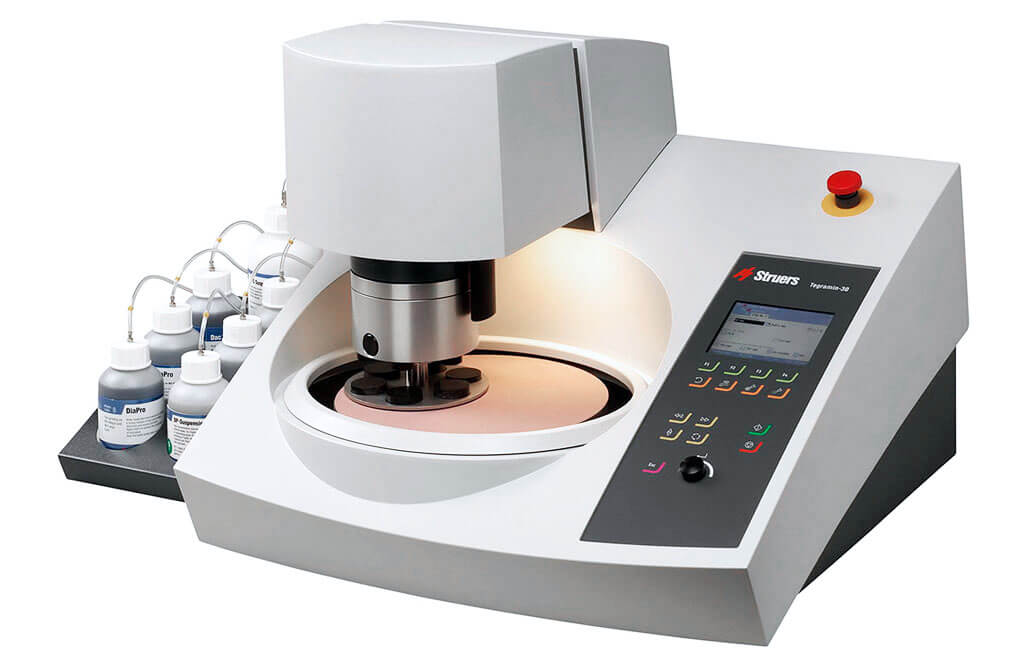
\includegraphics[width=0.5\textwidth]{fig/polishing/Tegramin.jpg}
    \caption{Struers Tegramin polishing machine}
    \label{fig:tegramin}
\end{figure}


\subsection{Stress and cracking}. 

Cracks forming in the core and cladding material was a problem encountered during polishing of the fibers. It is well documented that the as-drawn fibers contain stress \cite{Healy2018AFibres}, \cite{Fokine2017LaserFibers}, \cite{LapointeElectricalFibres}, \cite{KristinKristin_thesis_final}, but it remains an open question in the group whether the cracking observed during polishing results solely from thermal stress, or may also be caused by forces experienced during the polishing procedure. 
%Sources of Stress:
Stress is always formed in MCD fibers due to the different coefficients of thermal expansion of the core and cladding. There are further dynamics during the drawing process, including the interplay between the softening glass cladding and the expansion of the core as it solidifies that will effect the residual stresses in the fiber \cite{Healy2018AFibres}. This can lead to both tensile and compresive strain. Further post processing that reduces grain boundaries or transforms silicon from the amorphous to crystaline state will reduce the volume of the core and modify the stress \cite{Zhao2017EffectFibre}. The use of interface modifiers prevents a strong bond from forming between the Si and Si02 cladding which can reduce the strain in these cases \cite{Gibson2013AlkalineFibers}. 
Control of these stresses through laser annealing of the core has been used to create bandgap modification of Si  \cite{Healy2014ExtremeFibres} and to directly write bragg gratings into the fiber core \cite{Fokine2017LaserFibers}. Work by Zhao has shown that the stresses are concentrated in a ring near the core cladding interface \cite{Zhao2018EffectsFiber}. It was found that furnace annealing led to a reduction in stress, with greater reduction for increasing temperature. However these results should be treated carefully when comparing to our fibers as the as-drawn fibers used in this study were shown to have a low degree of crystallinity, and no interface modifier was used. The improvements in crystalinity of the core shown after the annealing process could be a factor leading to the reduction in stresses that may not be found in highly crystaline samples. However, heating the glass above the glass transition temperature and allowing for a slower cooling time then experienced in the fiber draw should have some impact on the stresses.

Silicon core fibers where chosen to represent a range of core diameters and core cladding ratios. These fibers were heated in a muffle furnace to 1200 with a rate of ?, held for ? minutes and cooled with a  rate of ?. These fibers were then machine polished using diamond abrasive under the same conditions as the untreated fibers. 

As a further test of the polishing procedure thin Si wafers (specifics) were mounted in epoxy and machine polished with the same parameters. Experimentally it was not possible to polish a wafer down to fiber dimensions, but the use of large wafers would expose any significant forces involved if they were to crack during polishing.

results: 


Annealing, Recrystalization, core-cladding ratio. %discussion on stress observations why less in redrawn fibers, annealed fibers?

\begin{figure}[h]
    \centering
    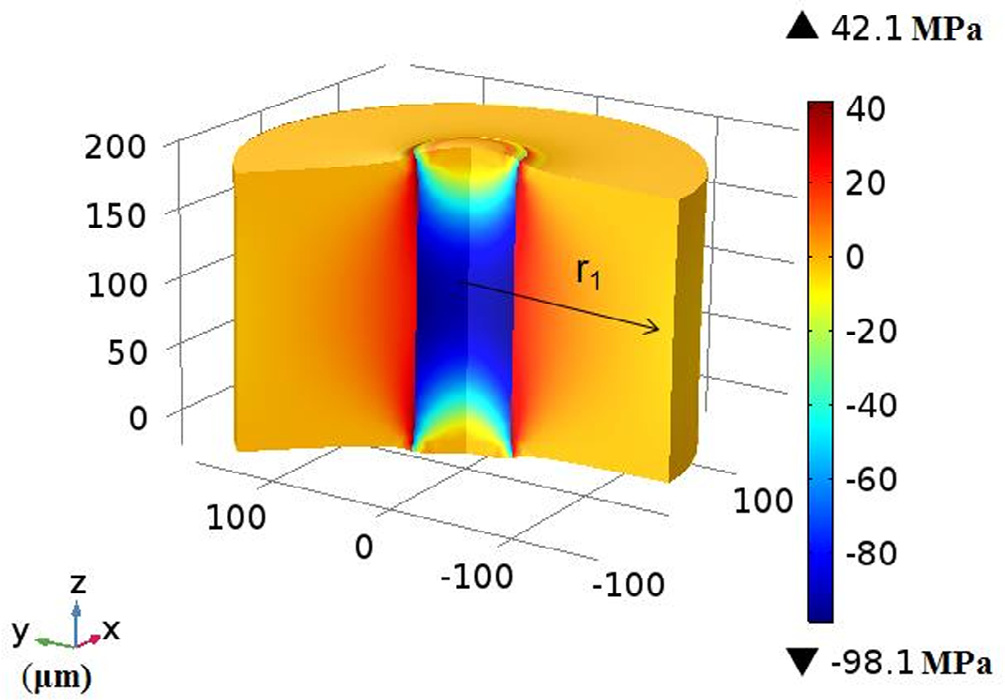
\includegraphics[width=0.5\textwidth]{fig/polishing/stress_simulation.png}
    \caption{Simulated results of stress in a Silica clad Germanium core fibre with no interface modifier, showing how stress may be distributed in a fiber. The core is $70\si{\micro\meter}$ and cladding $310\si{\micro\meter}$. Reprinted from \cite{Zhao2017EffectFiber}}
    \label{fig:my_label}
\end{figure}


\begin{figure}[h]
 %h here H requires float, exactly here, h! overide latex
\centering
\begin{subfigure}{.7\textwidth}
  \centering
  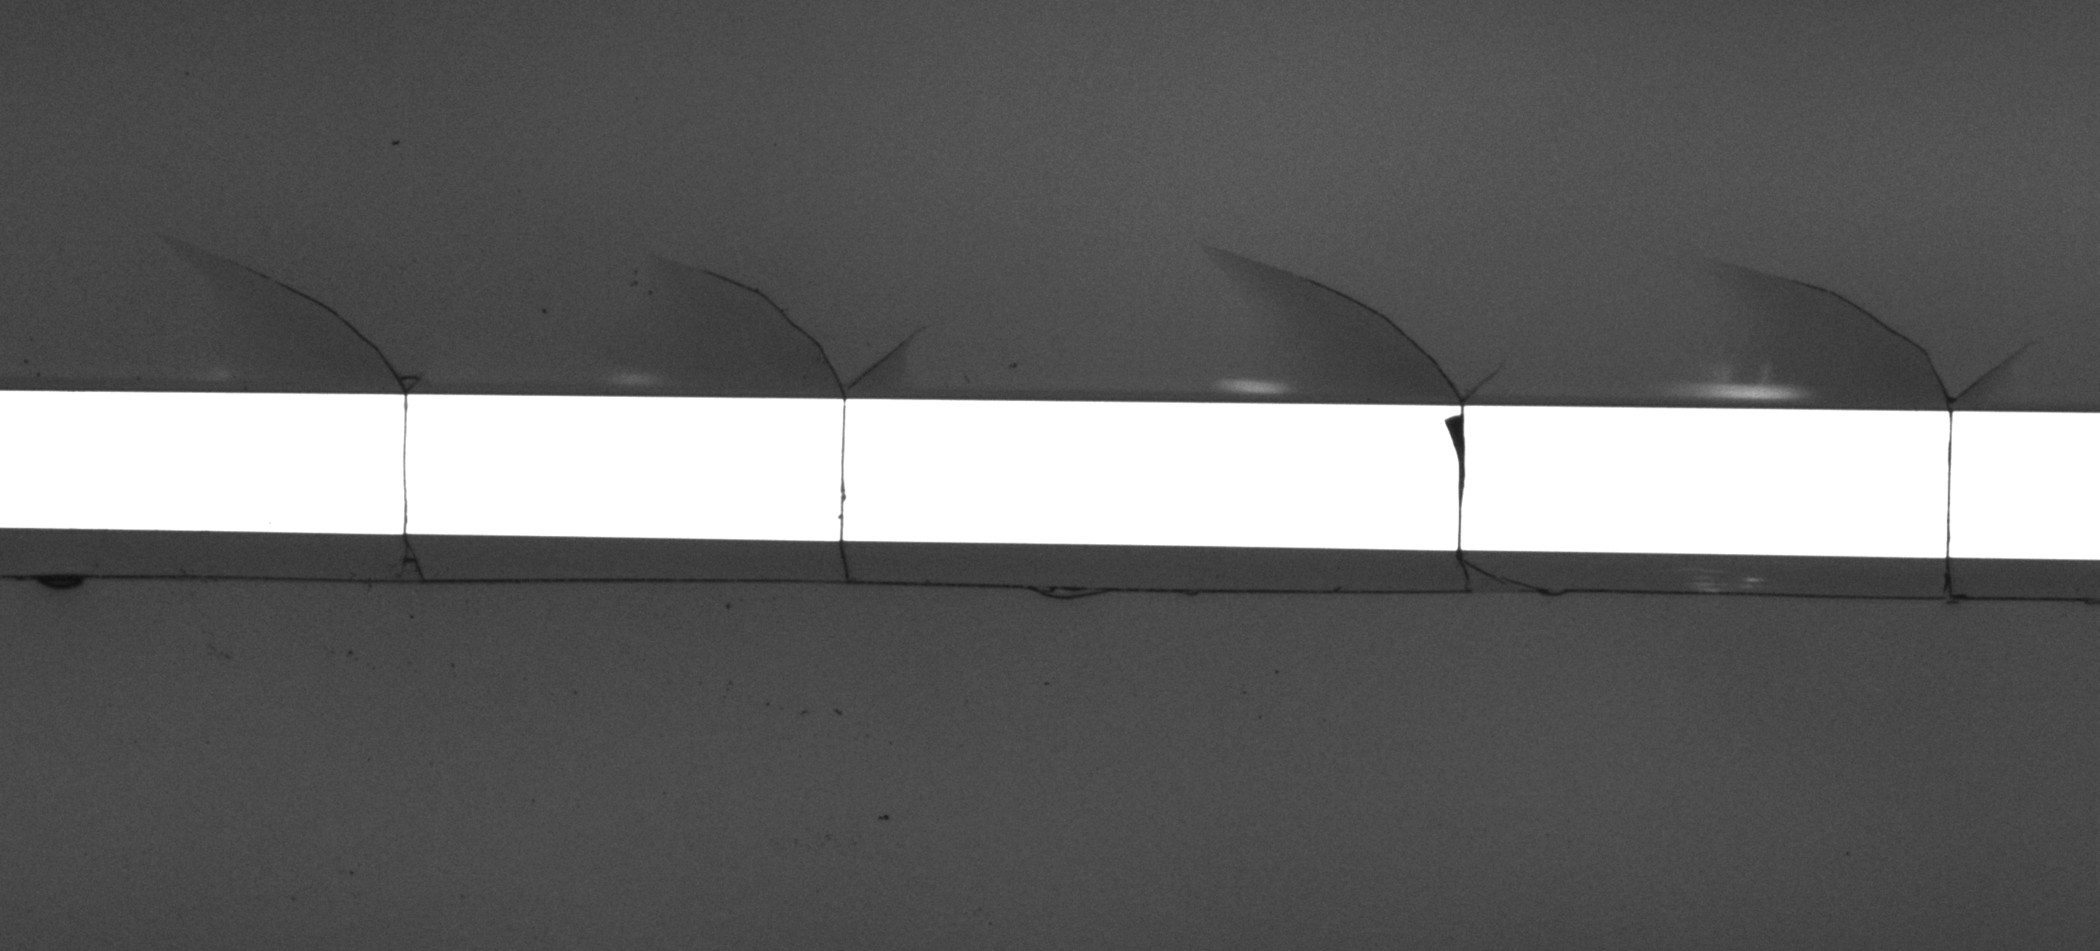
\includegraphics[width=\linewidth]{fig/polishing/Siedit.jpg}
  %\caption{1a}
  \label{fig:sfig1}
\end{subfigure}% %blank line makes figures vertical

\begin{subfigure}{.7\textwidth}
  \centering
  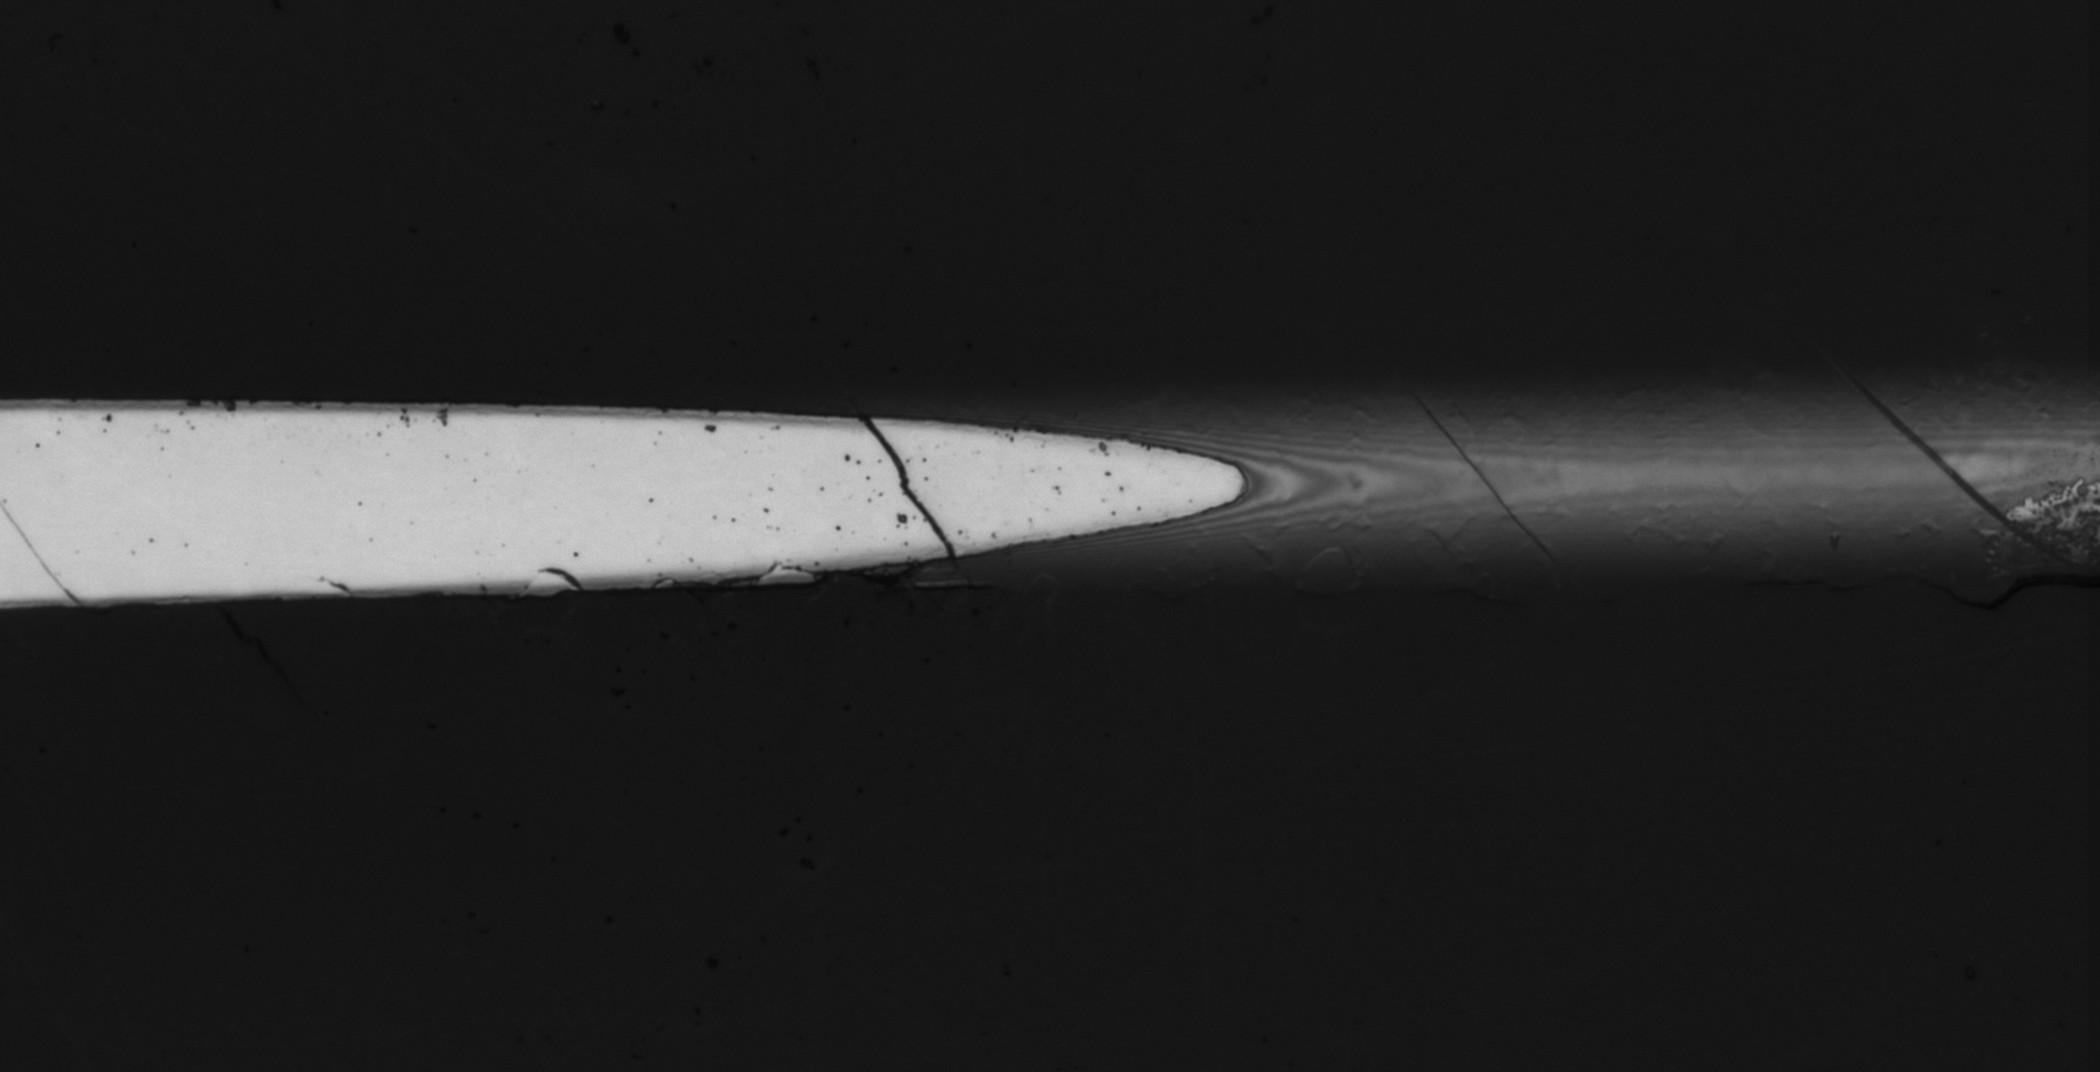
\includegraphics[width=\linewidth]{fig/polishing/SiGe.jpg}
  %\caption{1a}
  \label{fig:sfig2}
\end{subfigure}% %blank line makes figures vertical

\begin{subfigure}{.7\textwidth}
  \centering
  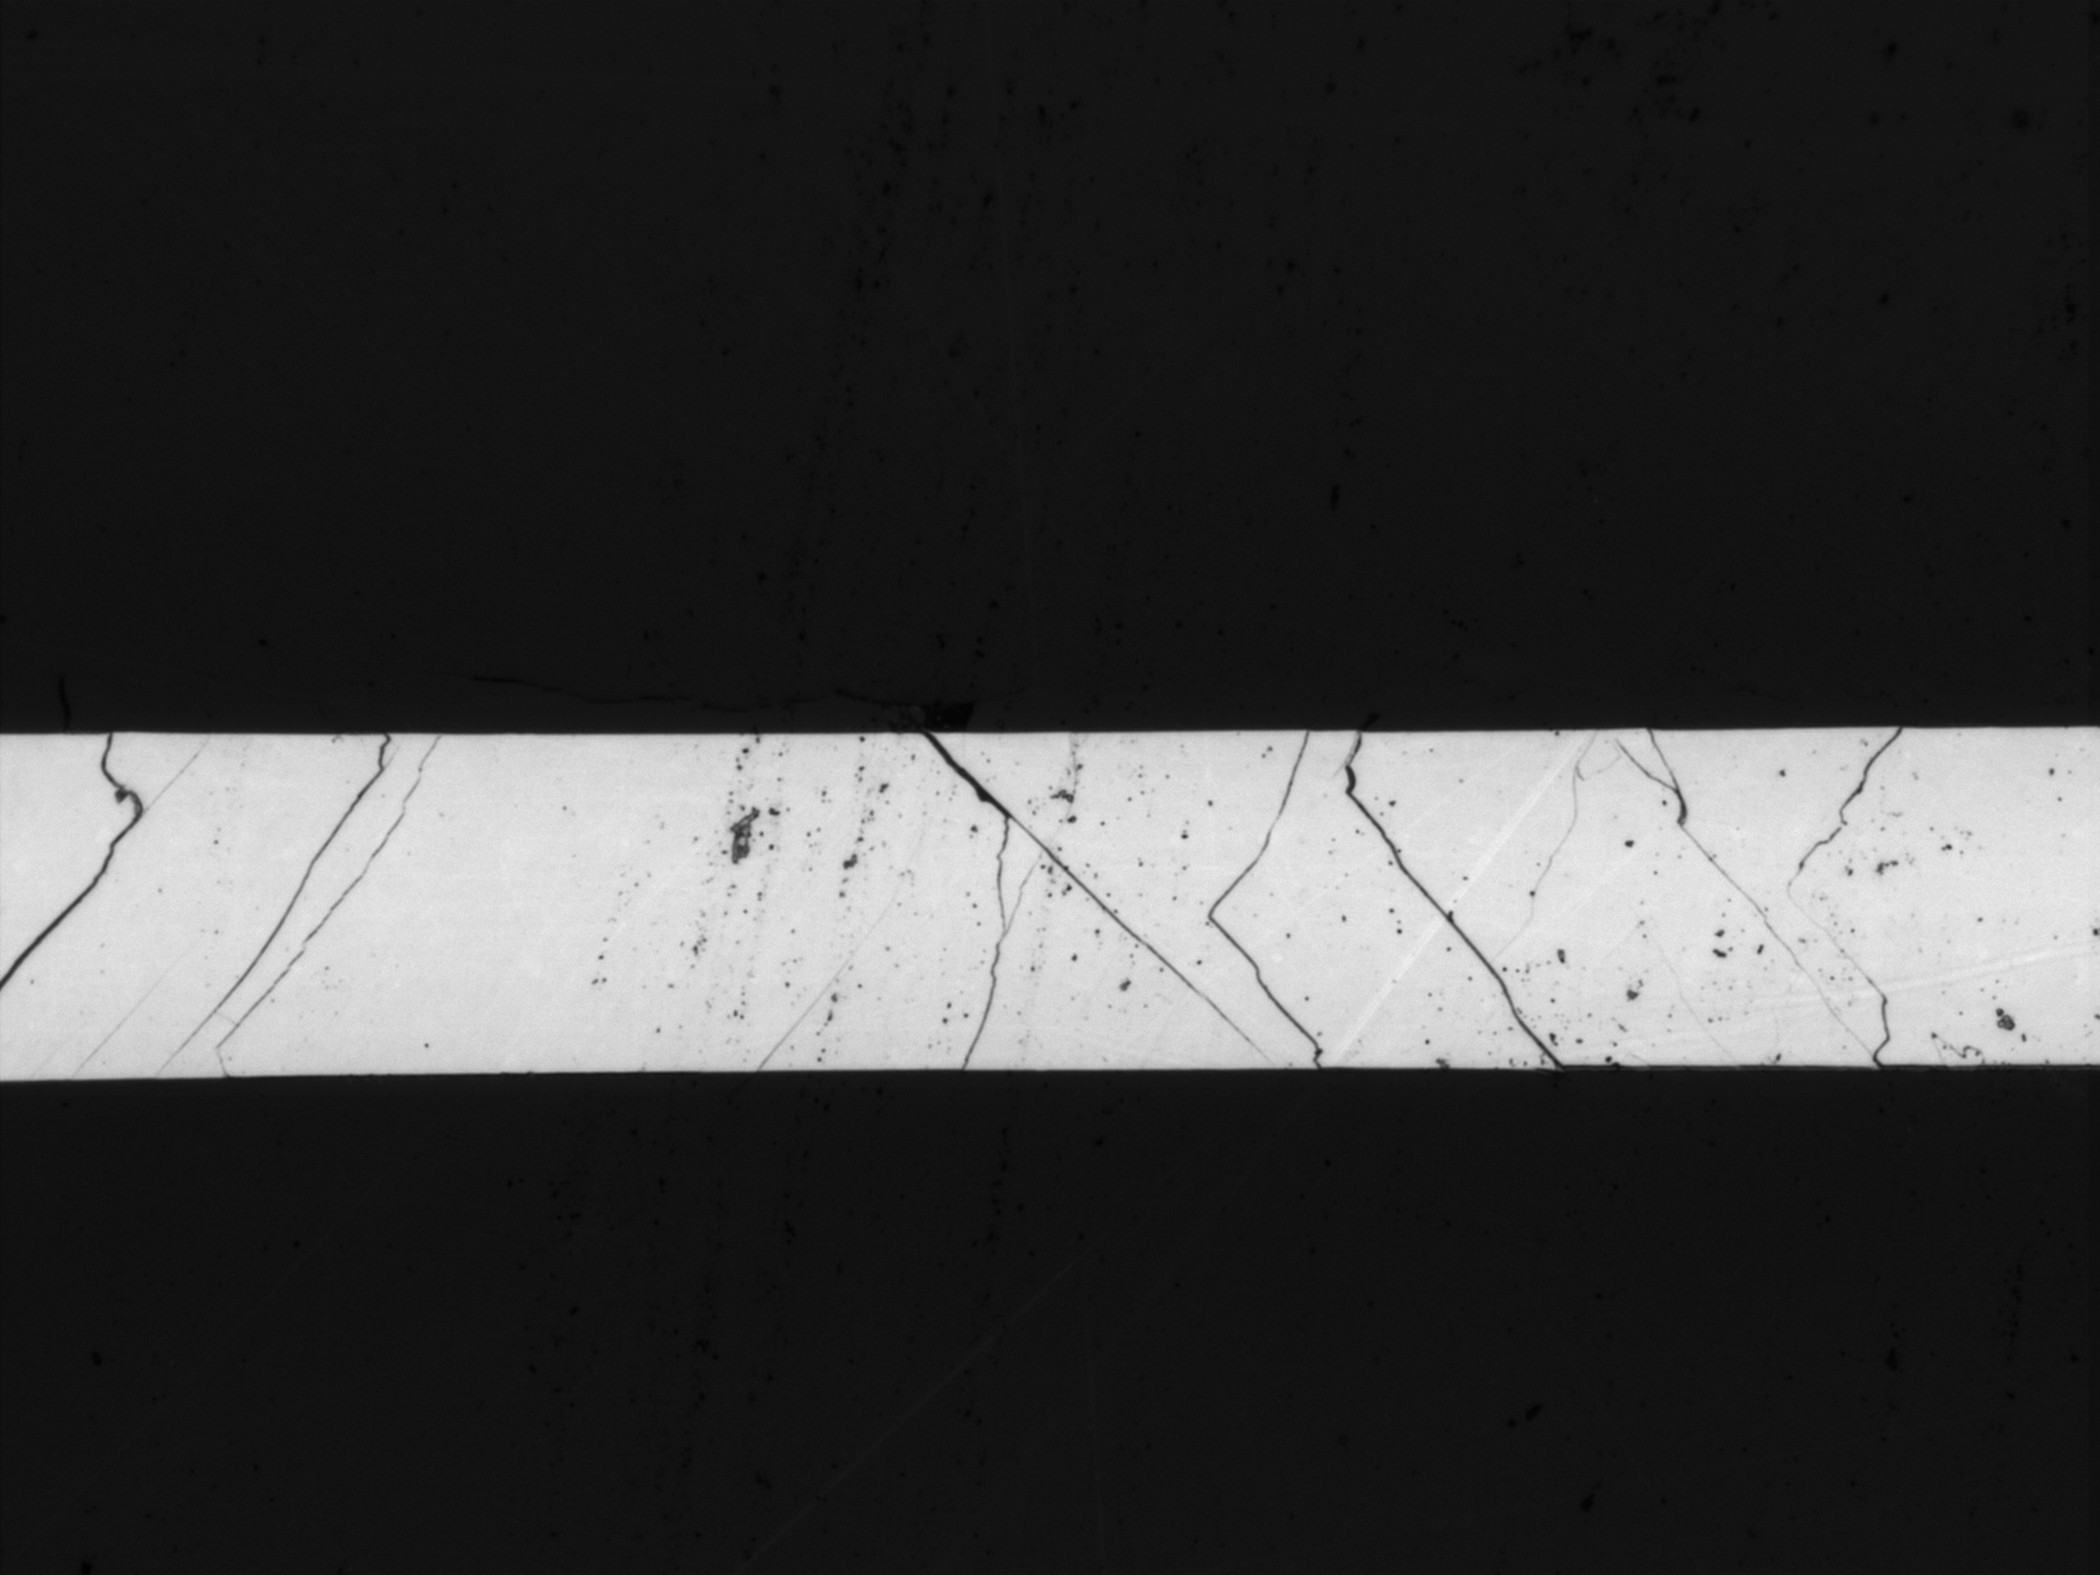
\includegraphics[width=\linewidth]{fig/polishing/SiGe2.jpg}
  %\caption{1b}
  \label{fig:sfig3}
\end{subfigure}
\caption{}
\label{fig:si_sige}
\end{figure}


\begin{figure}[h]
 %h here H requires float, exactly here, h! overide latex
\centering
\begin{subfigure}{.7\textwidth}
  \centering
  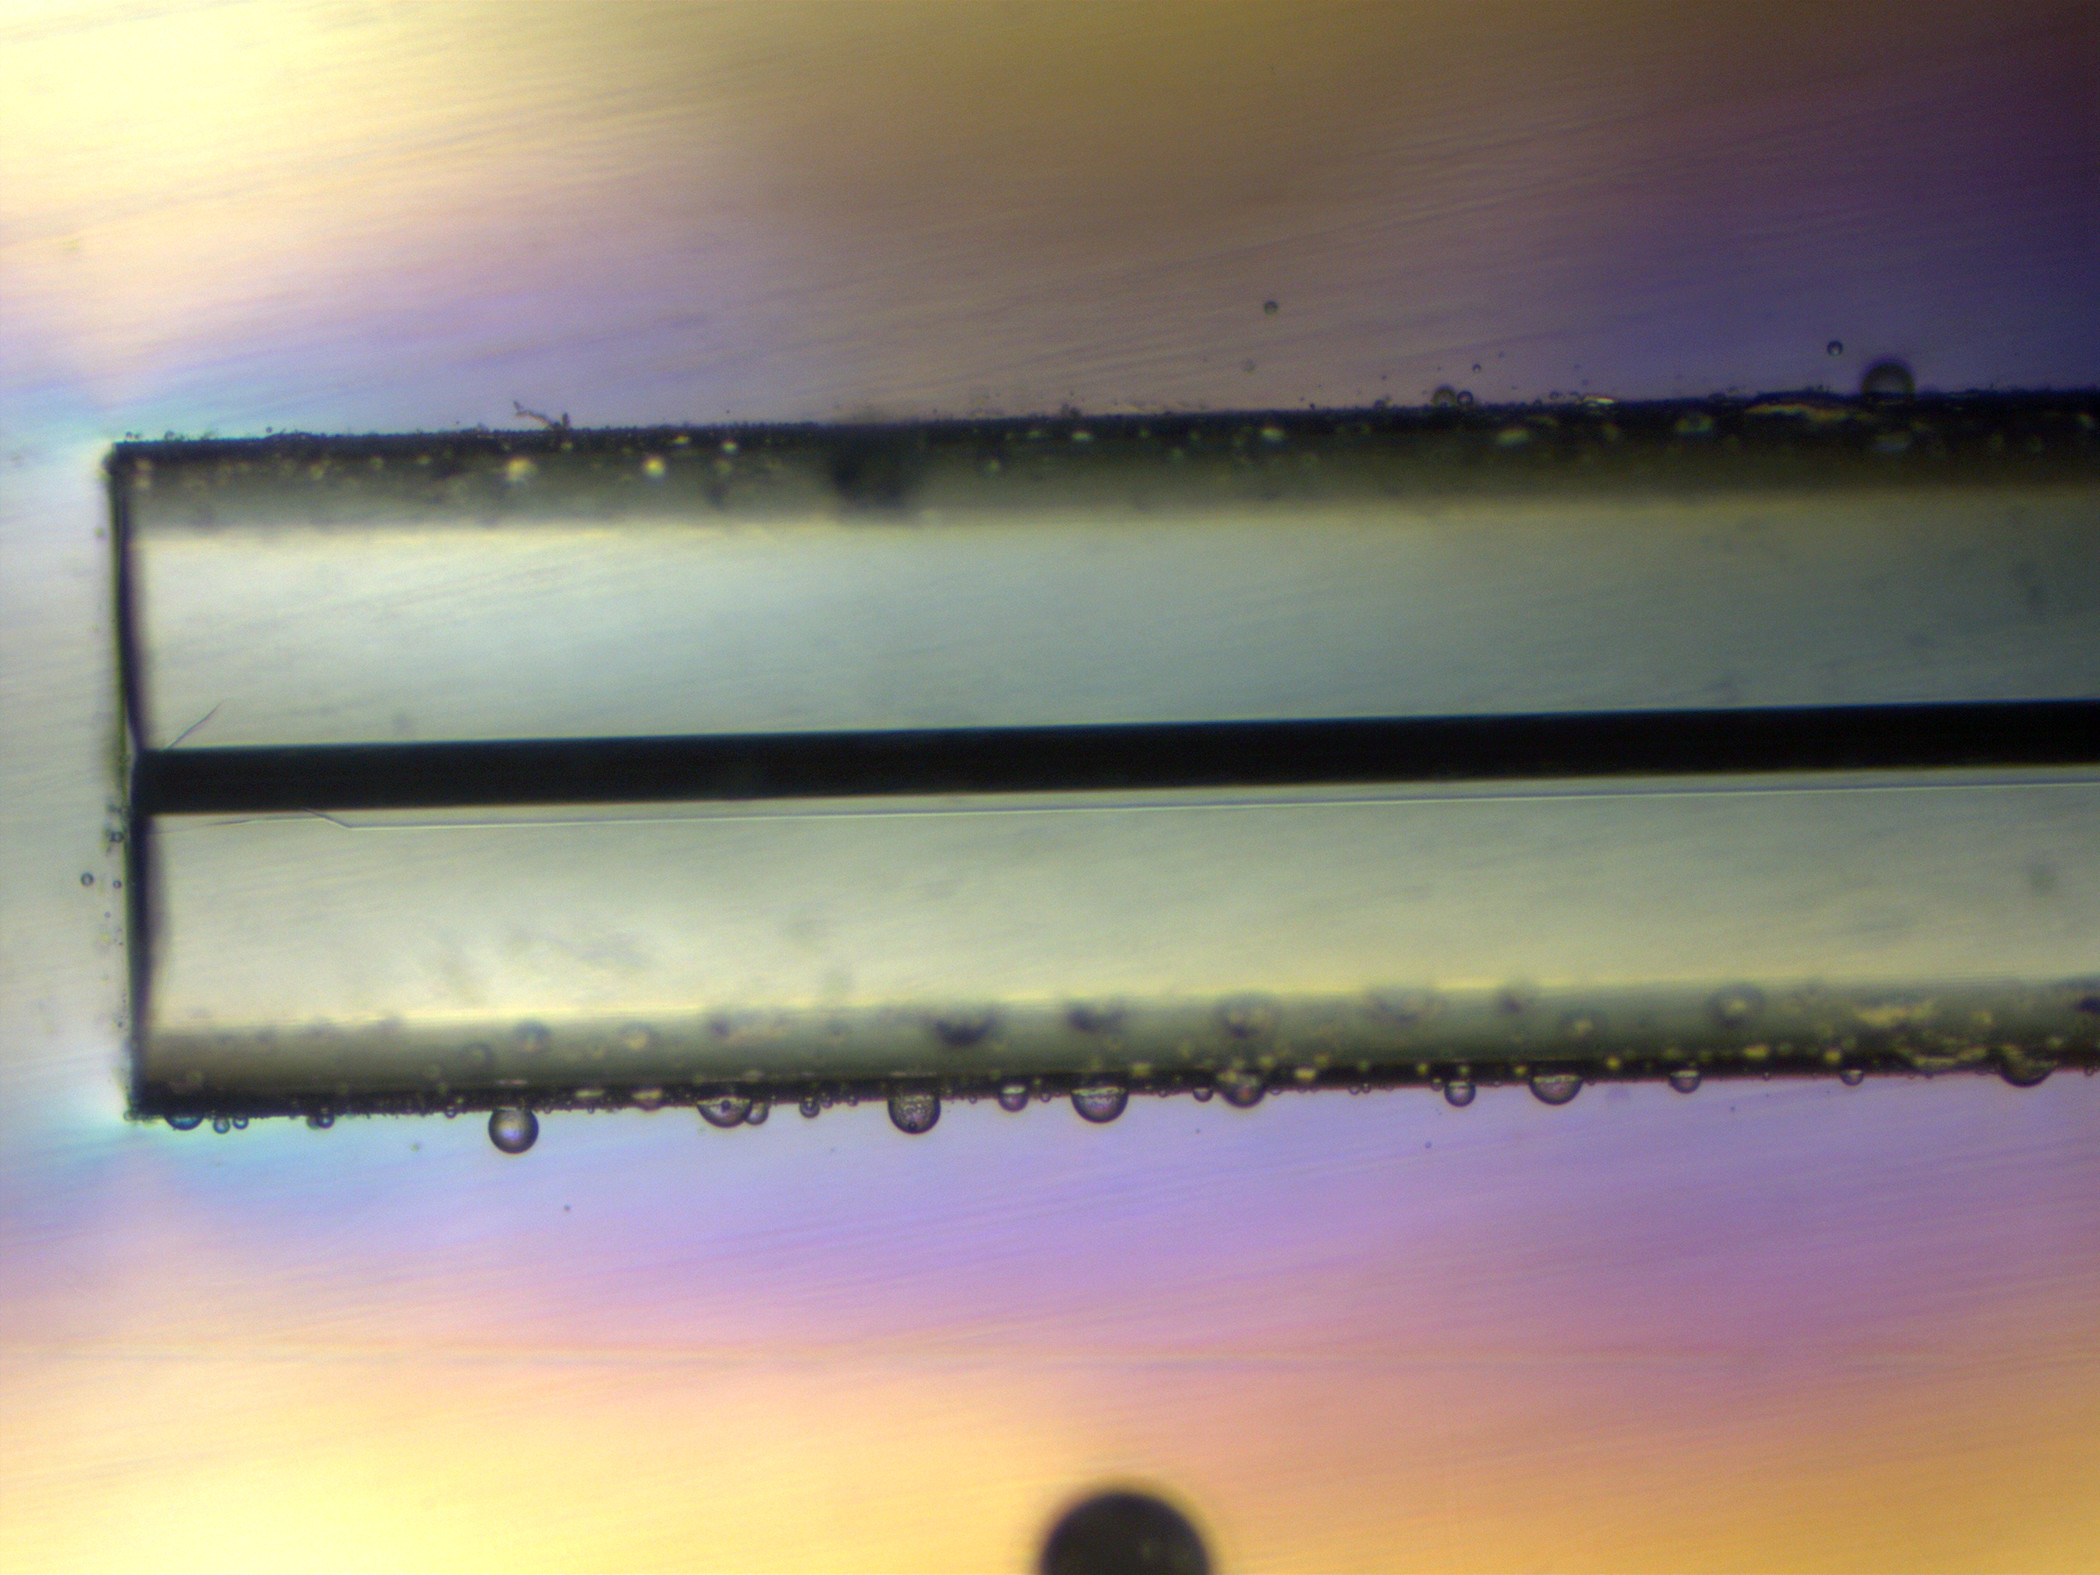
\includegraphics[width=\linewidth]{fig/polishing/parallelcrack.jpg}
  %\caption{1a}
  \label{fig:sfig1}
\end{subfigure}% %blank line makes figures vertical

\begin{subfigure}{.7\textwidth}
  \centering
  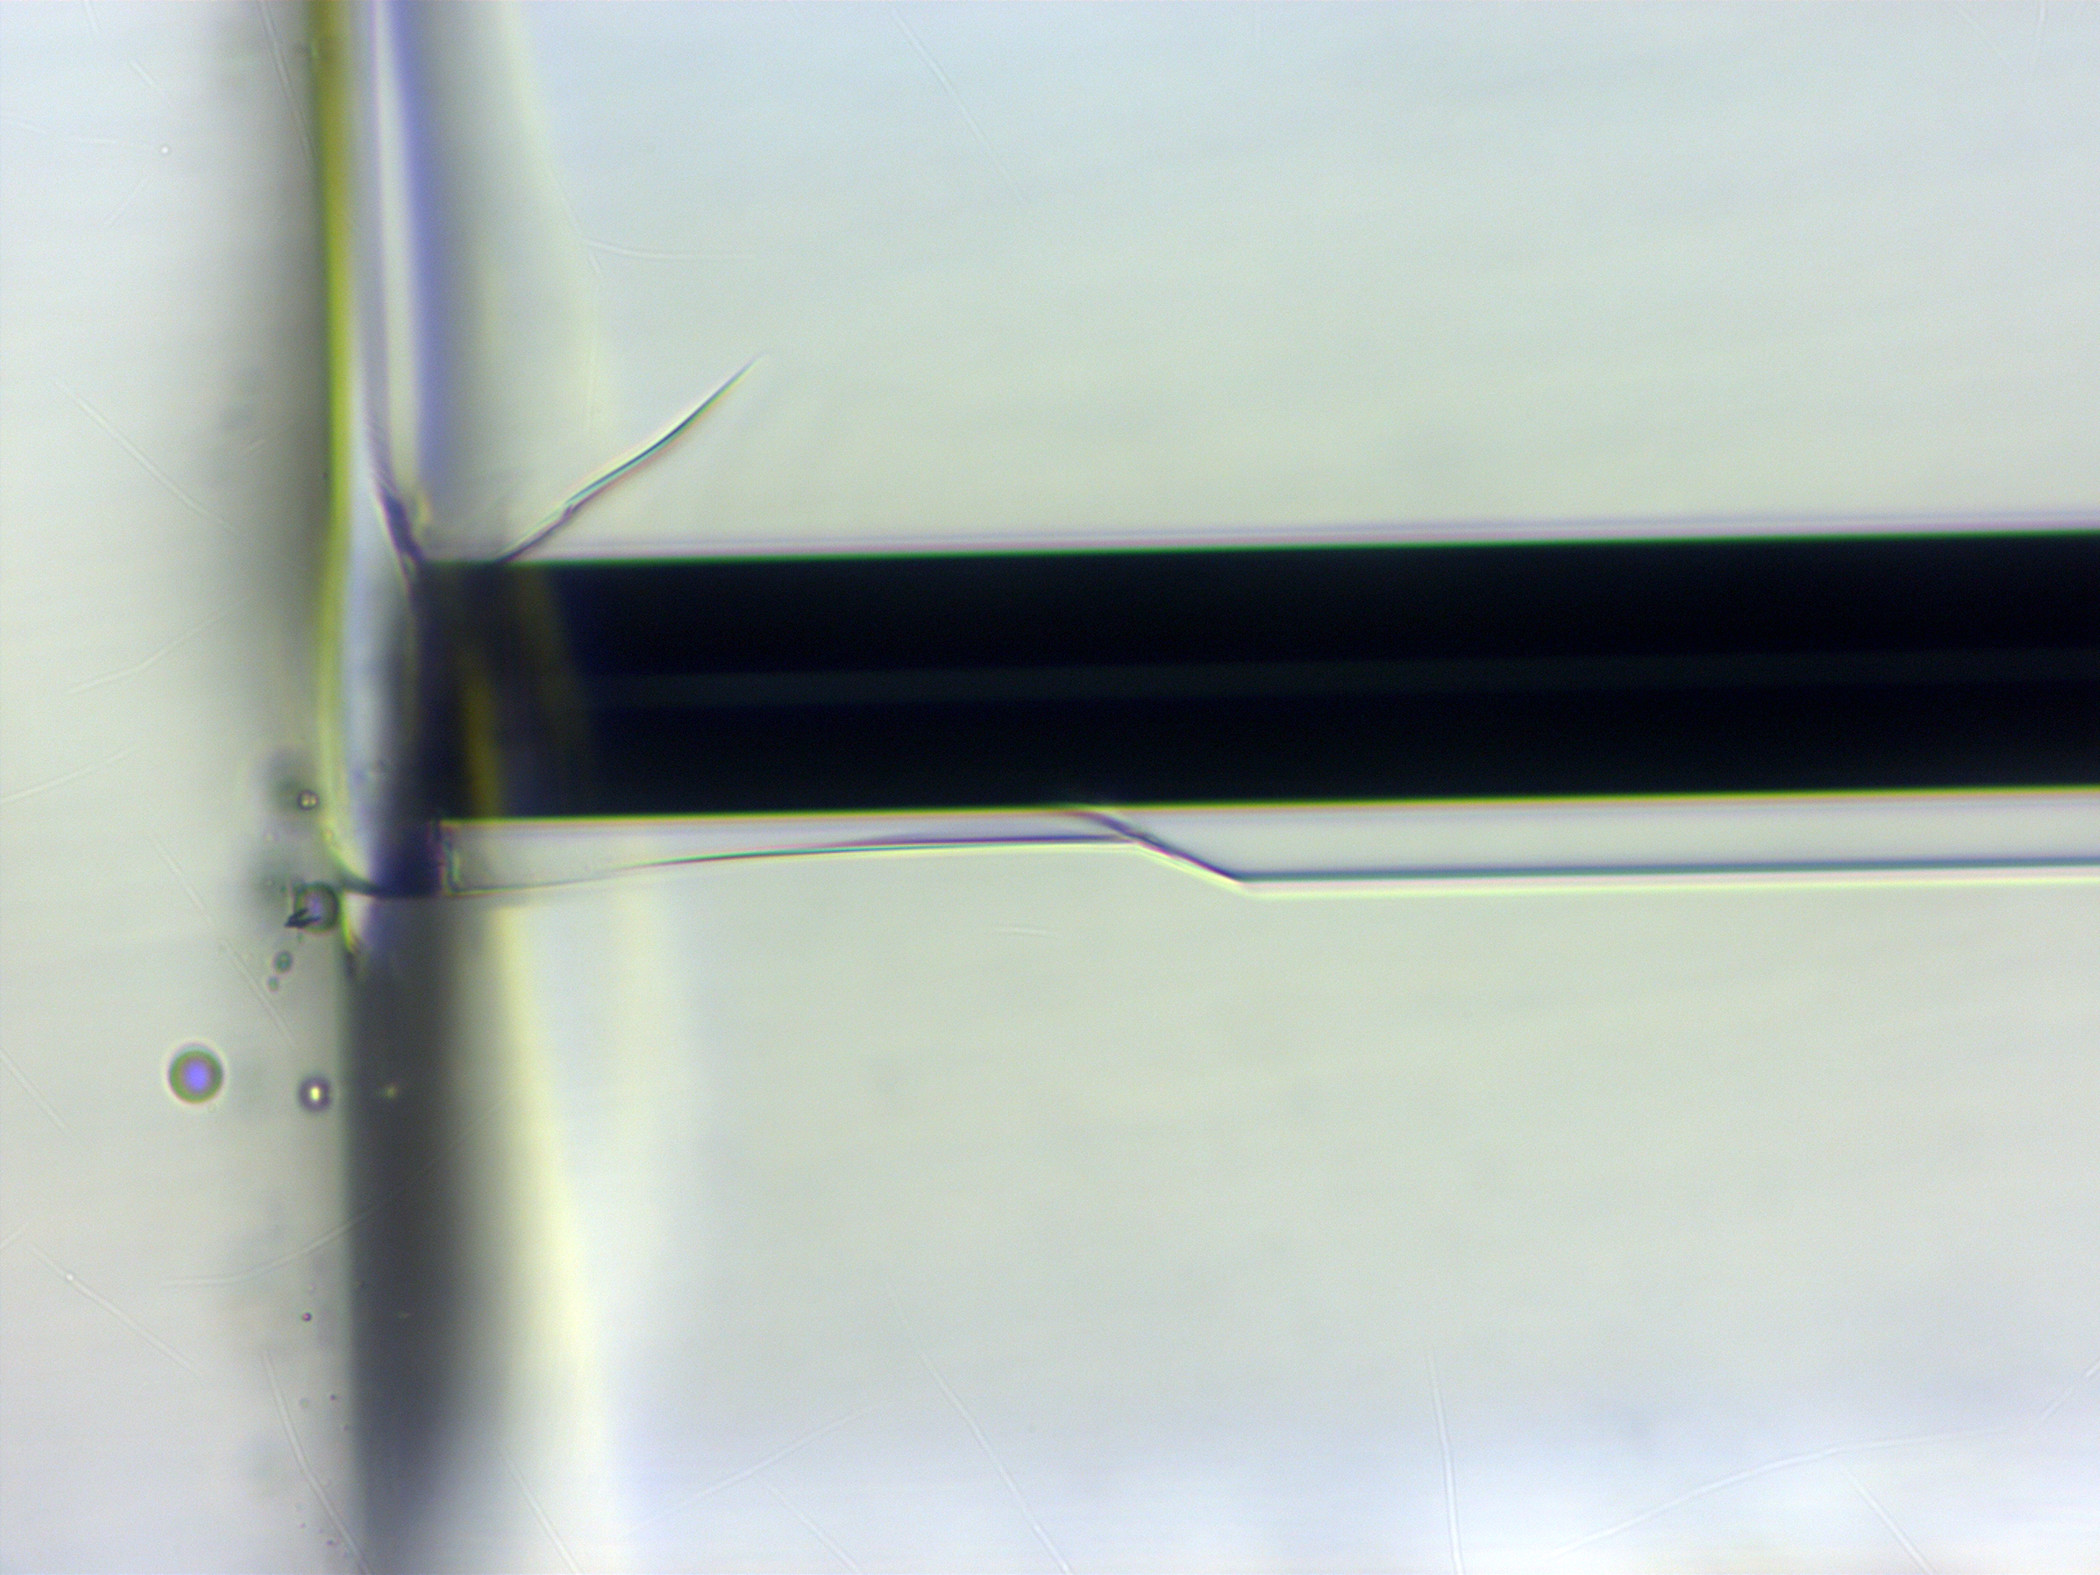
\includegraphics[width=\linewidth]{fig/polishing/parallelcrack2.jpg}
  %\caption{1a}
  \label{fig:sfig2}
\end{subfigure}% %blank line makes figures vertical

\begin{subfigure}{.7\textwidth}
  \centering
  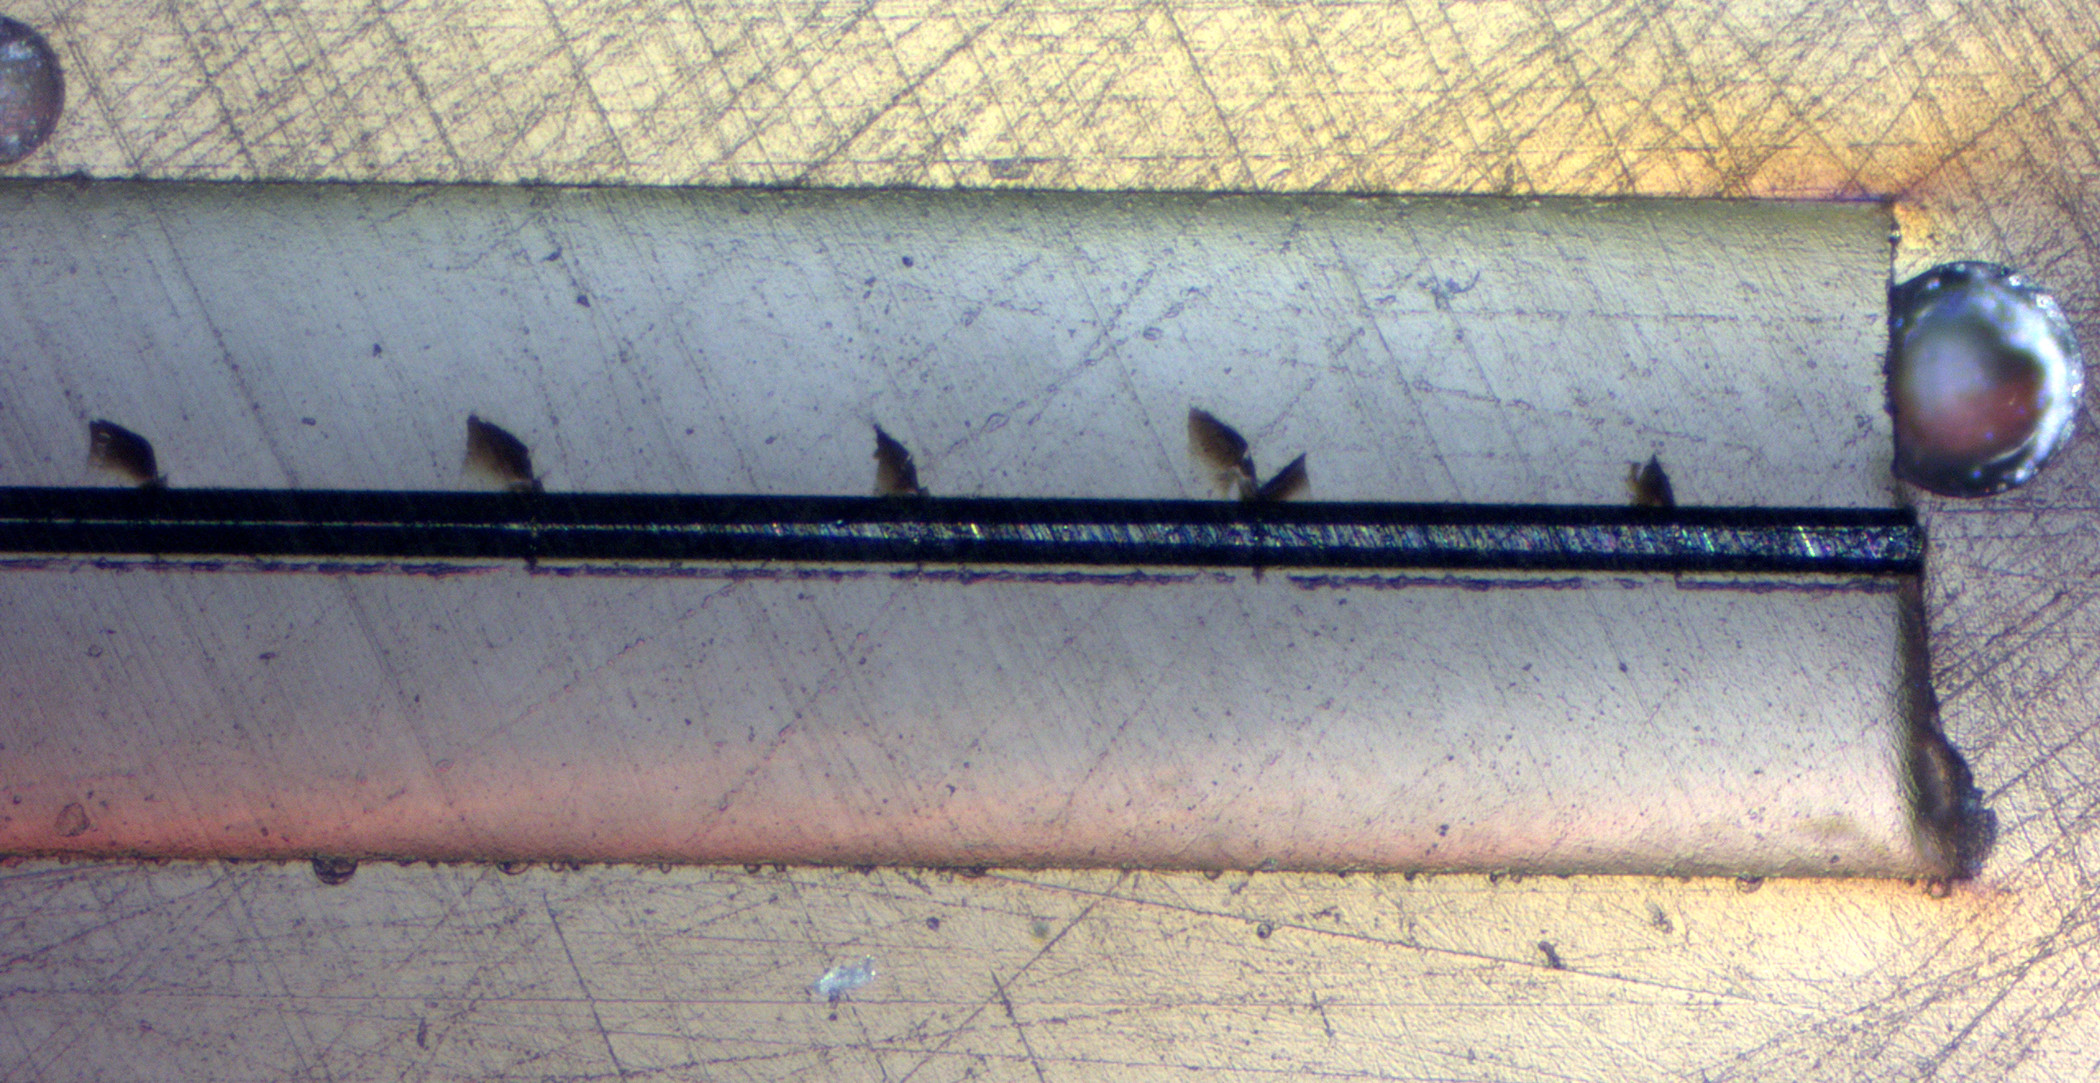
\includegraphics[width=\linewidth]{fig/polishing/parallelcrack3.jpg}
  %\caption{1b}
  \label{fig:sfig3}
\end{subfigure}
\caption{}
\label{fig:si_sige}
\end{figure}

\subsection{oven anneal}
\begin{figure}[h]
 %h here H requires float, exactly here, h! overide latex
\centering
\begin{subfigure}{\textwidth}
  \centering
  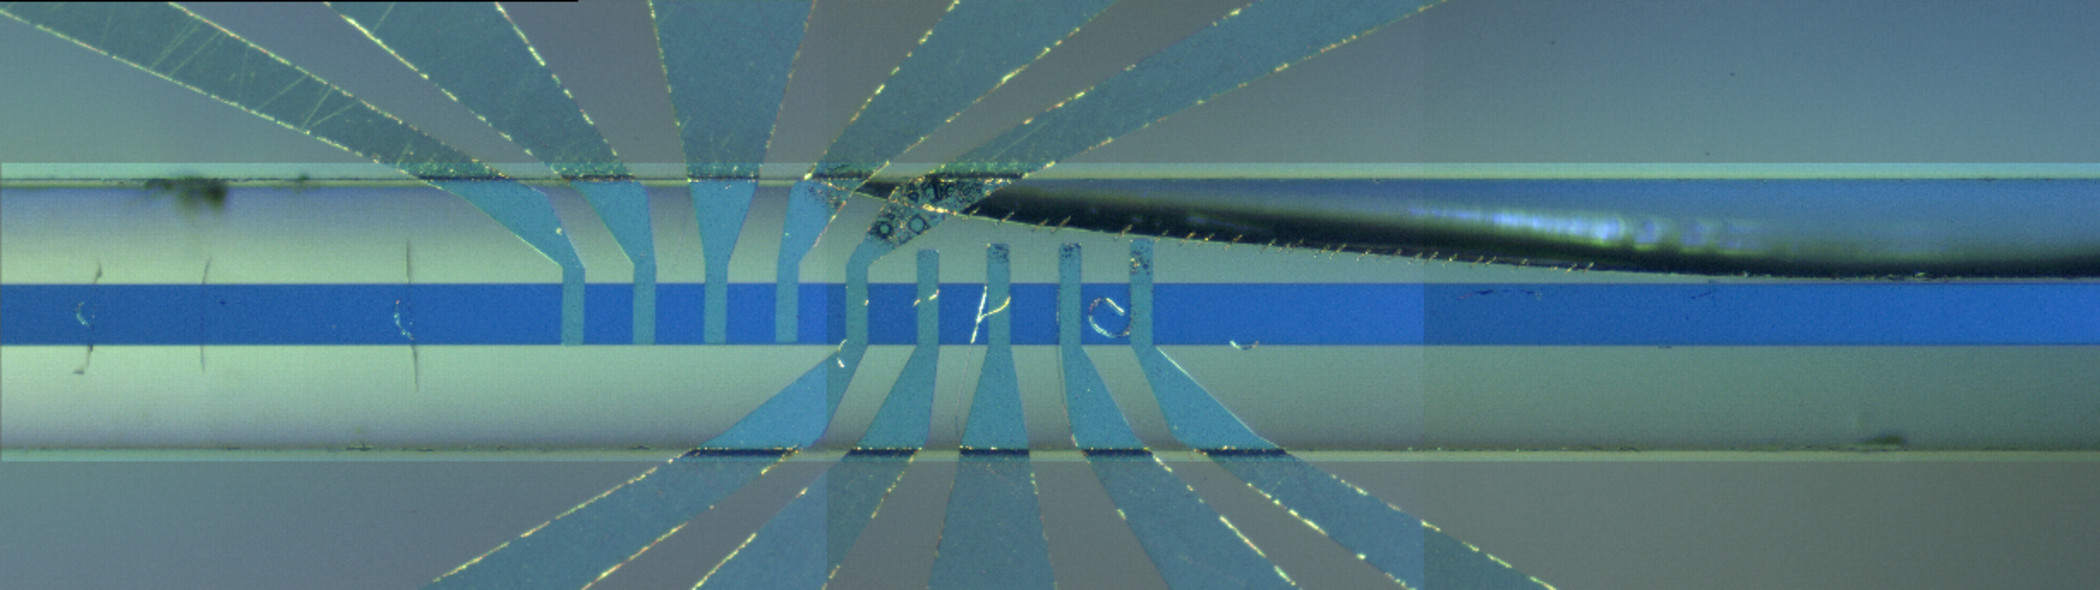
\includegraphics[width=\linewidth]{fig/OA/dd35114_0A--01-1.jpg}
  %\caption{1a}
  \label{fig:sfig1}
\end{subfigure}% %blank line makes figures vertical

\begin{subfigure}{\textwidth}
  \centering
  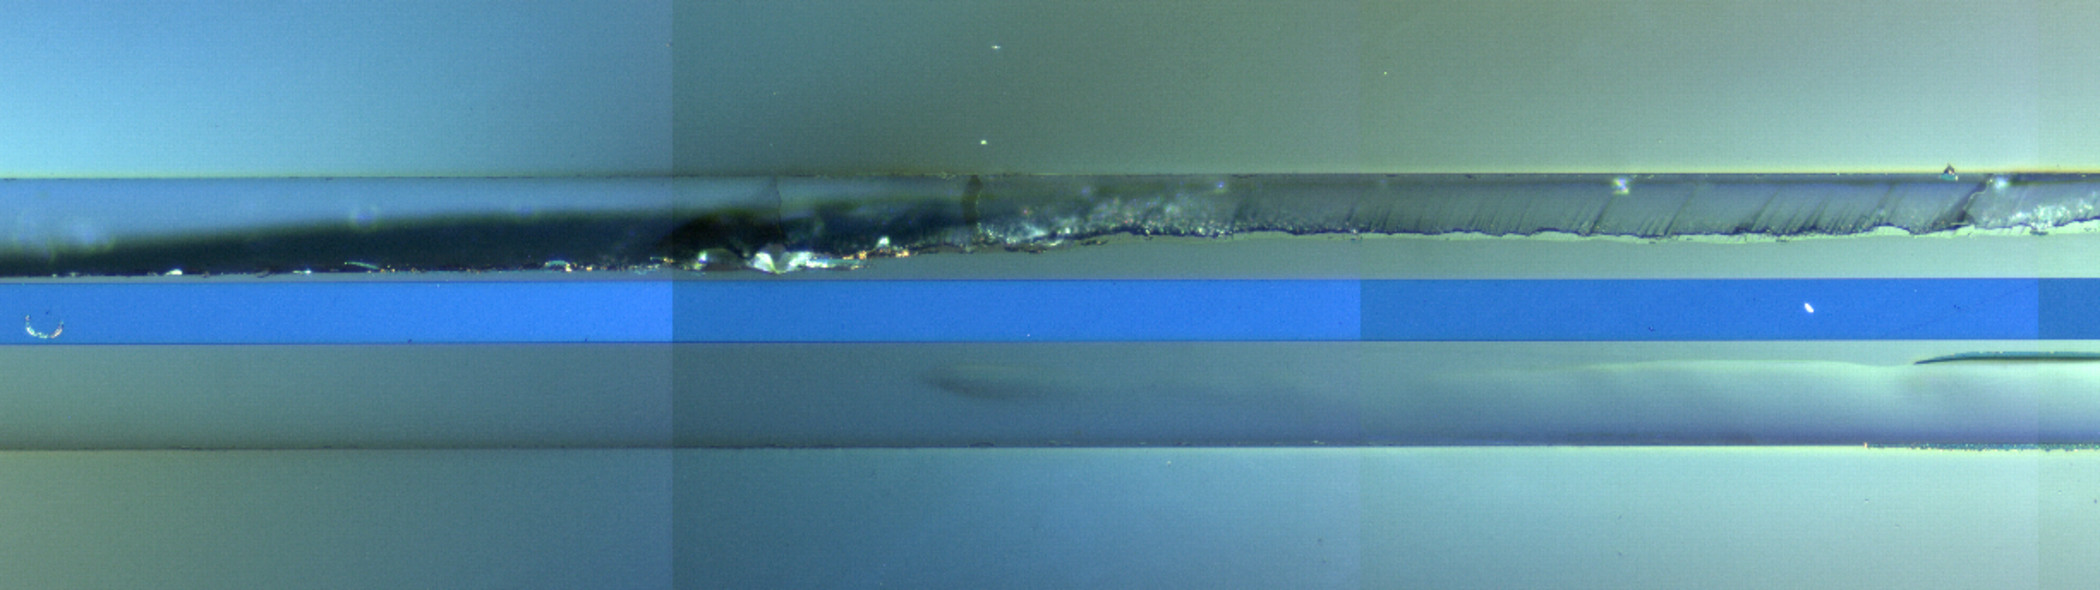
\includegraphics[width=\linewidth]{fig/OA/dd35114_0A--01-2.jpg}
  %\caption{1a}
  \label{fig:sfig2}
\end{subfigure}% %blank line makes figures vertical

\begin{subfigure}{\textwidth}
  \centering
  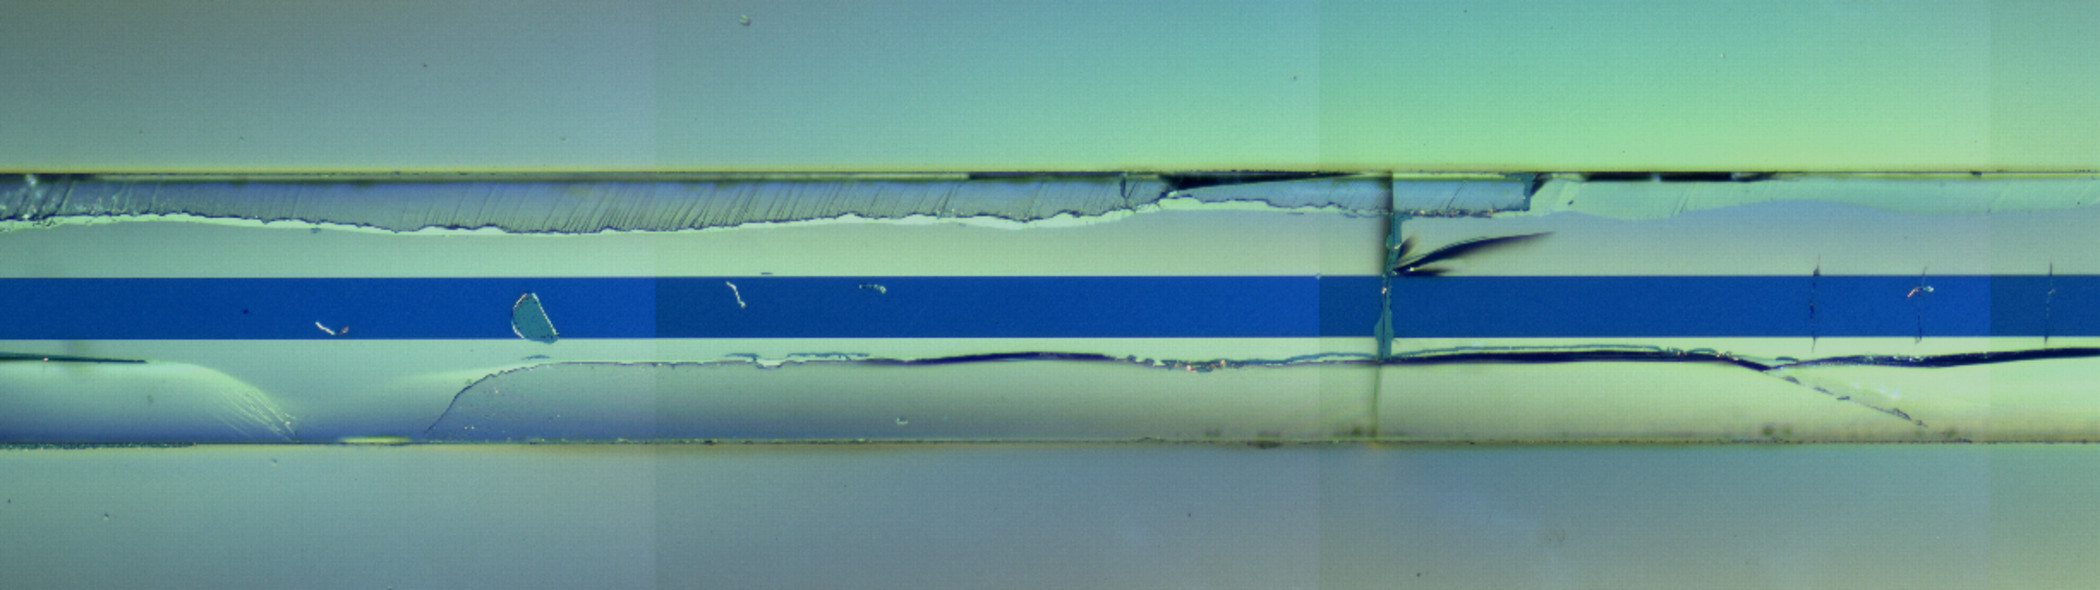
\includegraphics[width=\linewidth]{fig/OA/dd35114_0A--01-3.jpg}
  %\caption{1b}
  \label{fig:sfig3}
\end{subfigure}
\caption{Oven anneal Si fiber with ID dd35114 taken with a reflected light and polorization filter. Large cracks in the cladding, seem to act as a mechanism to relieve stress, as no cracking is observable in the core for these areas. Note due to image stiching, periodic vertical lines appear. }
\label{fig:si_sige}
\end{figure}

\begin{figure}
    \centering
    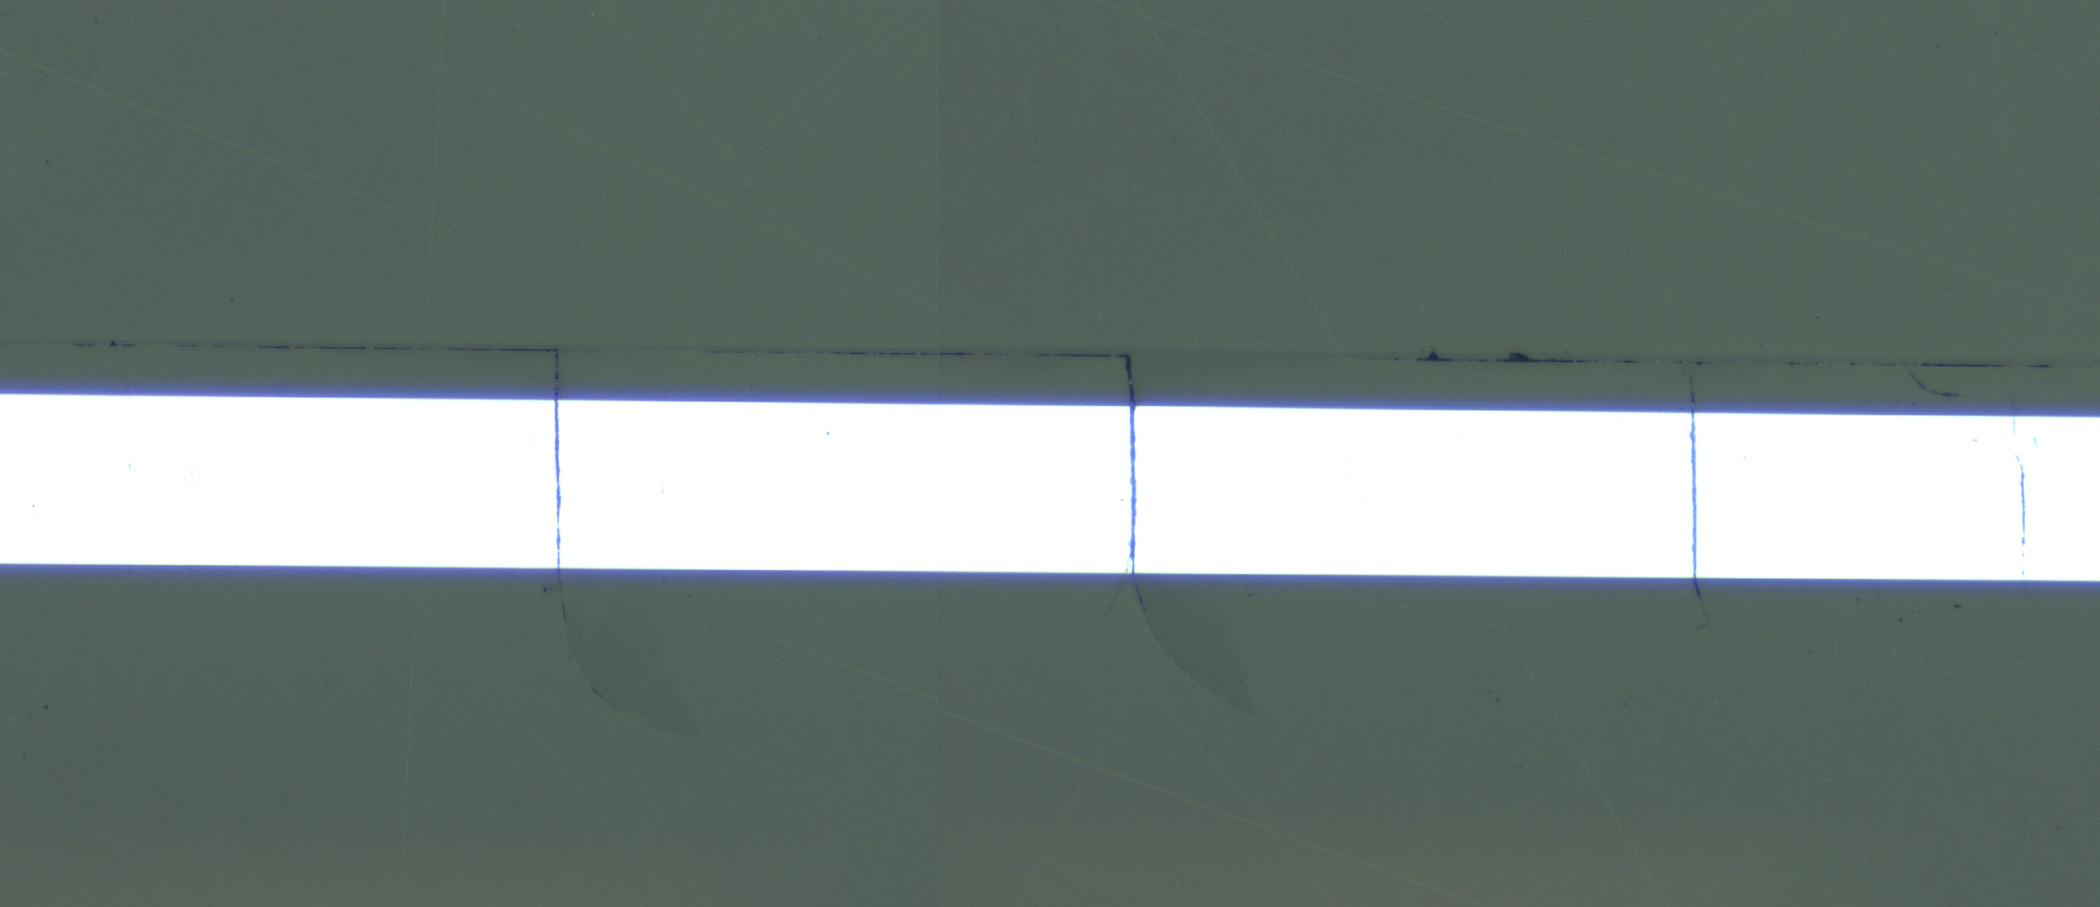
\includegraphics[width=\textwidth]{fig/polishing/dd354114_8.jpg}
    \caption{un annealed DD35114}
    \label{fig:my_label}
\end{figure}


\subsection{oven anneal}
\begin{figure}[h]
 %h here H requires float, exactly here, h! overide latex
\centering
\begin{subfigure}{\textwidth}
  \centering
  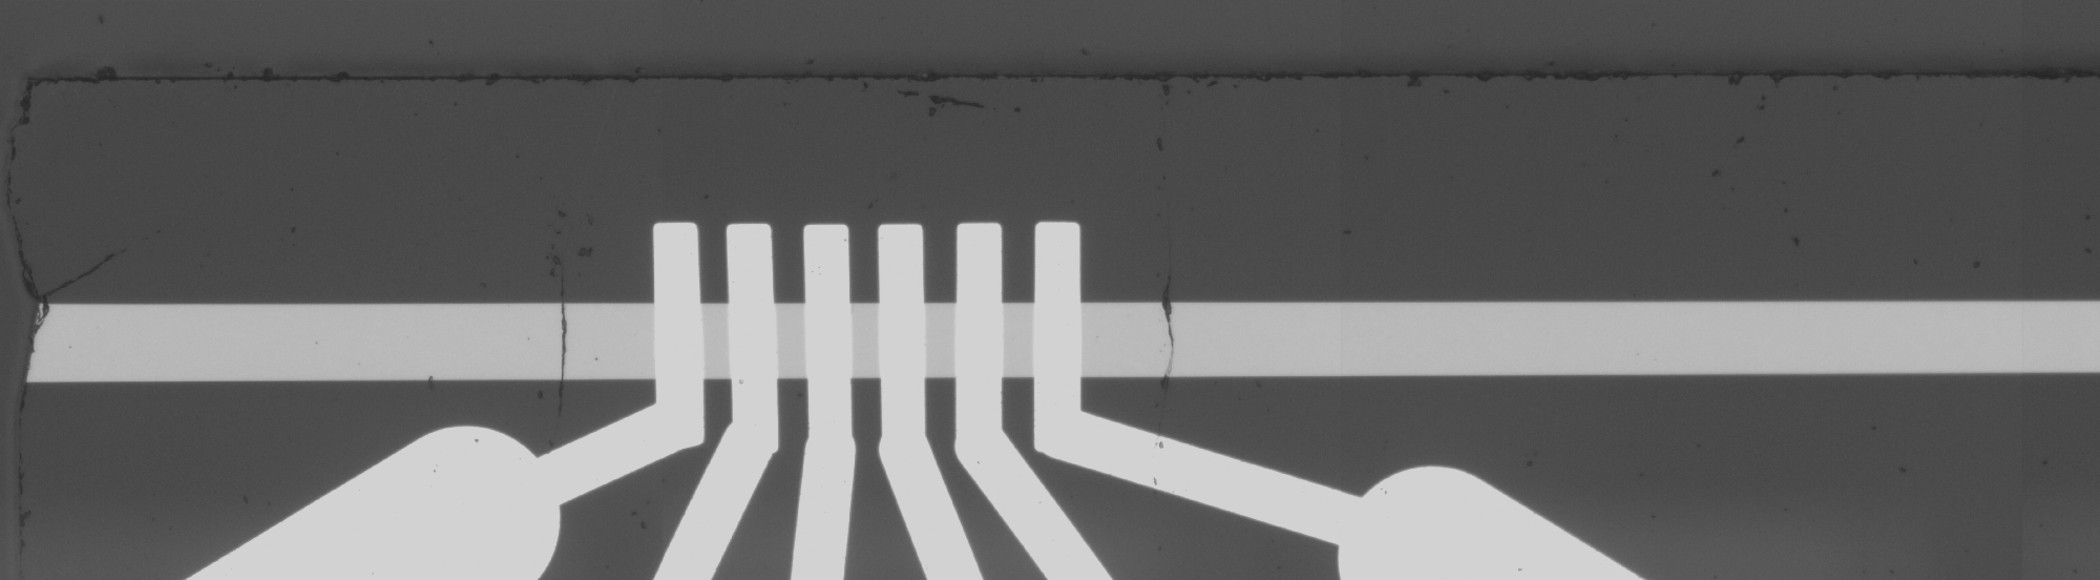
\includegraphics[width=\linewidth]{fig/OA/e944190422_redo-dup1.jpg}
  %\caption{1a}
  \label{fig:sfig1}
\end{subfigure}% %blank line makes figures vertical

\begin{subfigure}{\textwidth}
  \centering
  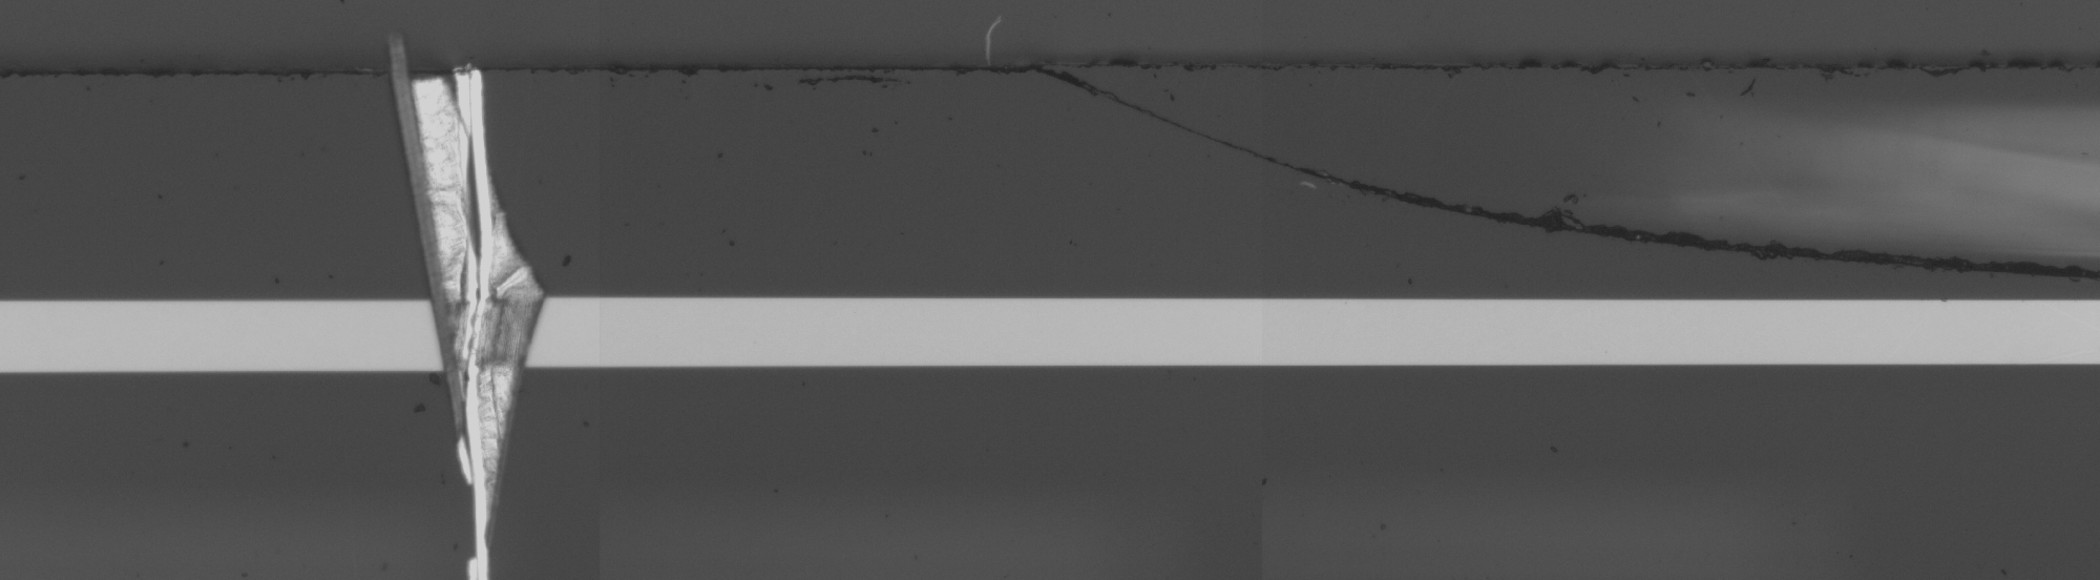
\includegraphics[width=\linewidth]{fig/OA/e944190422_redo-duplicate2.jpg}
  %\caption{1a}
  \label{fig:sfig2}
\end{subfigure}% %blank line makes figures vertical

\caption{Da13118 Annealed }
\label{fig:si_sige}
\end{figure}


\begin{figure}[h]
    \centering
    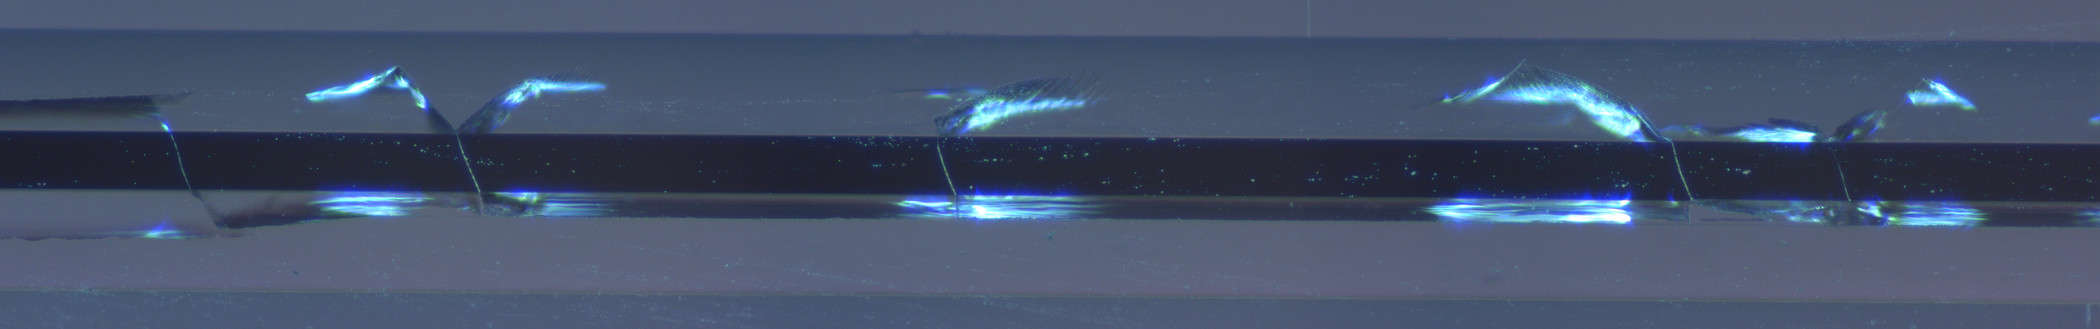
\includegraphics[width=\textwidth]{fig/polishing/e944.jpg}
    \caption{un annealed DA13118}
    \label{fig:my_label}
\end{figure}


\cleardoublepage